\usetikzlibrary{arrows.meta, calc, positioning}

\definecolor{weightblue}{RGB}{100,180,220}
\definecolor{reluorange}{RGB}{240,200,140}
\colorlet{skipred}{red!75!black}

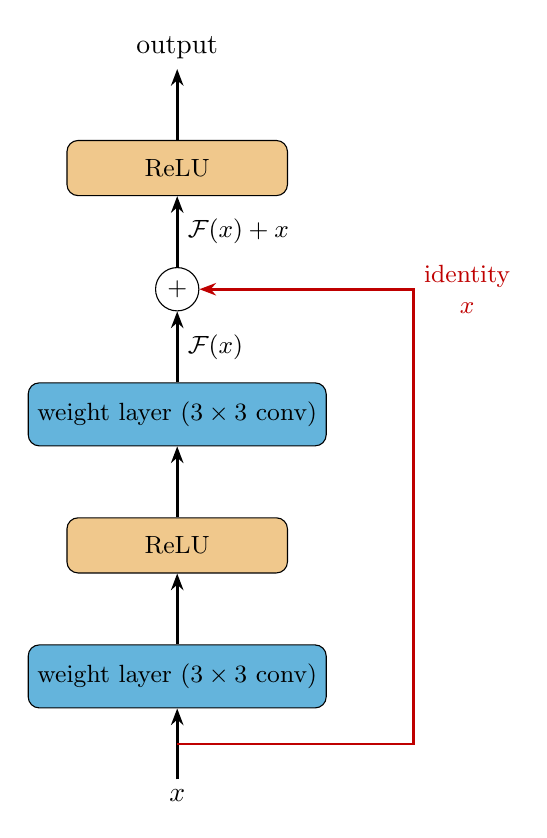
\begin{tikzpicture}[
    node distance=0.9cm,
    layer/.style={draw, rounded corners, fill=weightblue, minimum width=2.8cm, minimum height=0.8cm, font=\small},
    relu/.style={draw, rounded corners, fill=reluorange, minimum width=2.8cm, minimum height=0.7cm, font=\small},
    add/.style={draw, circle, minimum size=0.55cm, inner sep=0pt, font=\small},
    flow/.style={-{Stealth[length=6pt]}, line width=1pt},
    skip/.style={-{Stealth[length=6pt]}, line width=1pt, color=skipred},
]
% Main path, bottom to top
\node (x)    {$x$};
\node[layer, above=of x]    (w1)   {weight layer ($3\times3$ conv)};
\node[relu,  above=of w1]   (r1)   {ReLU};
\node[layer, above=of r1]   (w2)   {weight layer ($3\times3$ conv)};
\node[add,   above=of w2]   (plus) {$+$};
\node[relu,  above=of plus] (r2)   {ReLU};
\node[above=of r2]          (out)  {output};

% Main-path arrows
\draw[flow] (x)   -- (w1);
\draw[flow] (w1)  -- (r1);
\draw[flow] (r1)  -- (w2);
\draw[flow] (w2)  -- node[right, font=\small] {$\mathcal{F}(x)$} (plus);
\draw[flow] (plus) -- node[right, font=\small] {$\mathcal{F}(x) + x$} (r2);
\draw[flow] (r2)  -- (out);

% Identity skip connection (right side, bypassing both weight layers)
\coordinate (xtap) at ($(x.north)!0.5!(w1.south)$);
\draw[skip] (xtap) -- ++(3.0,0) coordinate (sk)
            |- (plus.east)
            node[skipred, midway, right, align=center, font=\small] {identity\\$x$} ;

\end{tikzpicture}
